\section{绪论}

\subsection{研究背景及意义}

21世纪后\cite{rendle2009bpr},隐身技术的发展促进了各国武器装备竞争的加剧,发展隐身技术,提高武器系统生存,空防和纵深打击能力,已经成为集陆、海、空、天、电磁五位一体的立体现代战争的迫切需要[1]。

针对不同的探测手段,隐身技术可分为雷达隐身技术、红外隐身技术、可见光隐身技术、激光隐身技术、声隐身技术和磁隐身技术等。对于飞行器而言,重点是雷达隐身和红外隐身[2]。随着隐身技术的发展,雷达散射截面积(RCS)缩减已经成为热门研究课题[3-5]。在RCS缩减的众多的方法中,雷达吸收材料(RAM)通过将入射电磁波转化为热量的方法得到广泛应用,近年来,人工复合材料兴起,如频率选择表面(Frequency Selective Surface,FSS)[6-7],电磁带隙(Electromagnetic Bandgap,EBG)表面[8],和超材料/超颖表面[9]提供了缩减RCS的另一种可能方法[10]。

频率选择表面(Frequency Selective Surface,FSS)是指完全相同的单元沿一维或二维方向周期排列而成的无限大阵列[11]。图1-1中给出了贴片型频率选择表面周期性阵列示意图,在实际应用中FSS必须依附在介质基板上或嵌入介质基板中。频率选择表面对某些频段的入射波呈现出全反射或者全投射的特性,从而有效地控制电磁波的传输与反射,其本质可近似一个空间滤波器。频率选择表面结构在现实中有各种应用如天线、雷达罩和反射天线[12]。当雷达进行探测任务时,雷达与飞机通常不属于同一个高度,此时雷达波会呈一个大角度入射到飞机表面。在平板型吸波结构的设计中,如何在大角度斜入射的情况下保持其吸波性能的稳定性成为一个重难点。
\begin{figure}[htbp]
	% caption放上面就会显示在图的上方,出现在下面就是出现在图的下方
	% label的位置也有讲究
	\begin{center}
		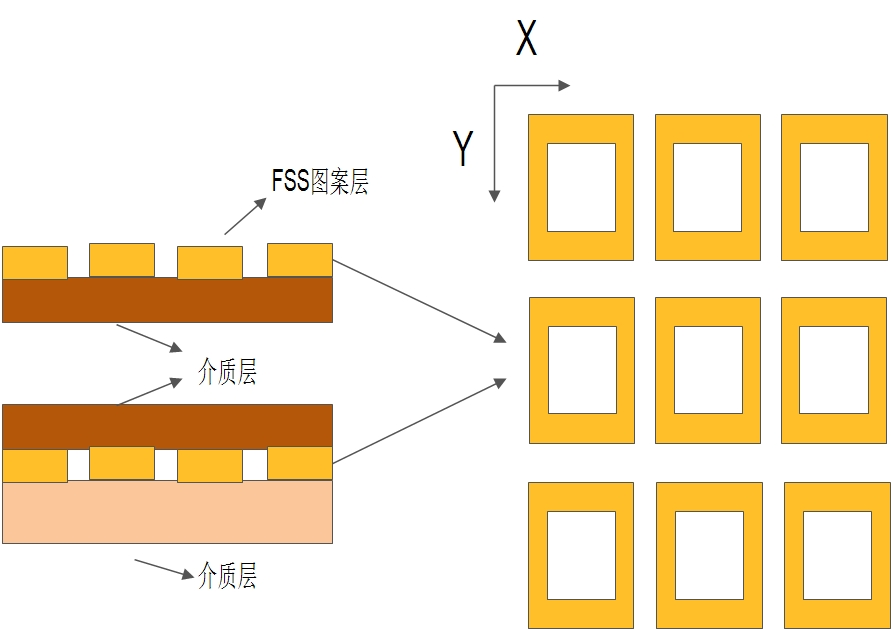
\includegraphics[width=1.0\textwidth]{fssstructure}
		\caption{FSS结构}
		\label{gra4}
	\end{center}
\end{figure}

\begin{figure}[htbp]
	\centering
	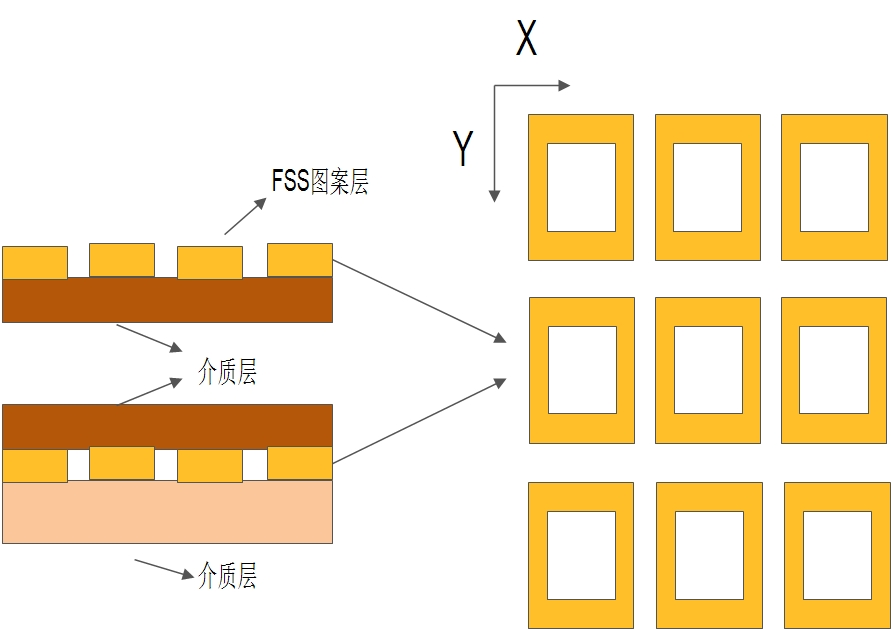
\includegraphics [width=1.0\textwidth]{fssstructure}
	\caption{南京理工电光13级}\label{dianguang13}
\end{figure}

\begin{equation}
    Recall_u = \frac{|\mathcal{I}_u^{re} \cap \mathcal{I}_u^{te}|}{|\mathcal{I}_u^{te}|}
    \end{equation}
\subsubsection{FSS}
\begin{equation}
    Recall_u = \frac{|\mathcal{I}_u^{re} \cap \mathcal{I}_u^{te}|}{|\mathcal{I}_u^{te}|}
	\end{equation}

	Google\footnote{\url{https://www.google.com/}}
